\section{Homepage} \label{Homepage}
Un sito web possiamo paragonarlo ad un negozio. Prima di entrare in un nuovo negozio l’approccio comune consiste nel guardare la vetrina. Questo è un punto cruciale, perché é proprio in quel momento che decidiamo se entrarci o proseguire oltre. Questo avviene per il web esattamente allo stesso modo. La homepage in questo contesto é la vetrina del negozio. \\
Arrivati quindi alla vetrina bisogna fornire all'utente nel minor tempo possibile le informazioni che sta cercando o  suscitare la sua curiosità. Il proprietario del sito web deve pertanto cercare di soddisfare le cosiddette 6 W, descritti in \hyperref[Assi informativi]{Sezione \ref{Assi informativi}}. 

\begin{figure}[H]
	\centering 
	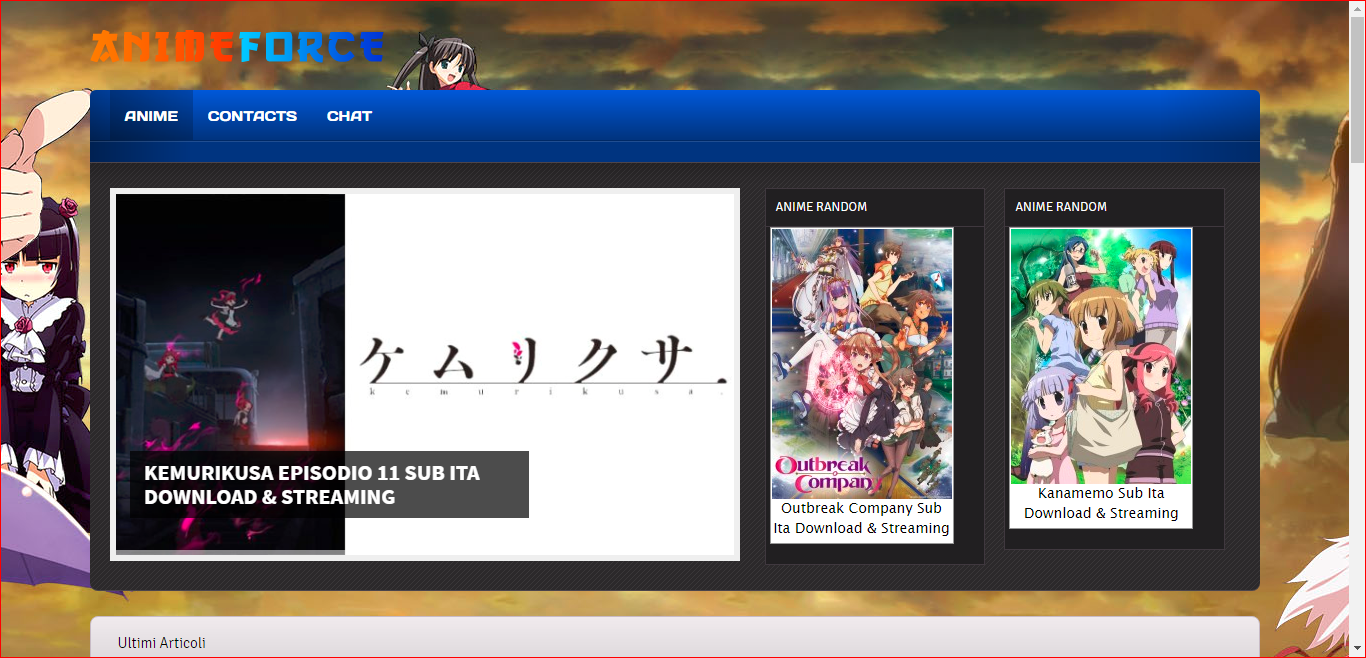
\includegraphics[width=1\textwidth]{img/hp01.png}
	\caption{Homepage} 
	\label{img1} 
\end{figure}

\subsection{I 6 assi informativi} \label{Assi informativi}

\subsubsection{Where - "A che sito sono arrivato?"} \label{HWhere}
Appena arrivati alla homepage, è riconoscibile,  in tempi non eccessivamente lunghi, che il sito si occupa di fornire streaming e download di anime. Ciò è possibile grazie alla presenza, negli unici testi presenti, delle parole "downolad \& Streaming". In questo modo é comprensibile a primo sguardo di cosa il sito tratta, per cui se una qualunque persona fosse interessata a guardare una serie animata giapponese potrebbe continuare la navigazione nel sito.

\subsubsection{Who - "Chi c'è dietro al sito?"} \label{HWho}
Le immagini presenti nella homepage fanno capire immediatamente agli appassionati del settore che il topic del sito sono gli anime (suggerito anche dal nome del sito analizzato in \hyperref[Nome]{Sezione \ref{Nome}}). Per un utente generico, invece, chiunque riconoscerebbe le immagini e le ricondurrebbe alla categoria dei cartoni animati. I tempi di comprensione da questo punto di vista sono molto rapidi. La specifica di essere giapponesi è comprensibile da una parte del nome del sito, ma soprattutto dai titoli dei cartoni in uscita e recenti presentati attraverso uno slideshow. Quindi alla domanda "Chi c'è dietro al sito?" si può rispondere con un team che ha una passione per gli anime e desidera diffondere cultura in questo ambito.

\subsubsection{Why - "Perché dovrei dare la mia fiducia? Che benefici mi dà?"} \label{HWhy}
La pagina non presenta alcuna descrizione della sua offerta, procede con il mostrare una lista degli anime del momento e di quelli passati. Presuppone che l'utente sia arrivato alla pagina con l'intento di guardarsi un anime, o in generale ottenere delle informazioni su di esso. Questa comportamento da parte degli ideatori del sito non attira l'utente e non fornisce alcun elemento a cui poter dare fiducia. Sebbene vi siano utenti che ritornano, con un layout più "snello" e una descrizione nella homepage suppongo che il numero di "affezionati" potrebbe aumentare.

\begin{figure}[H]
	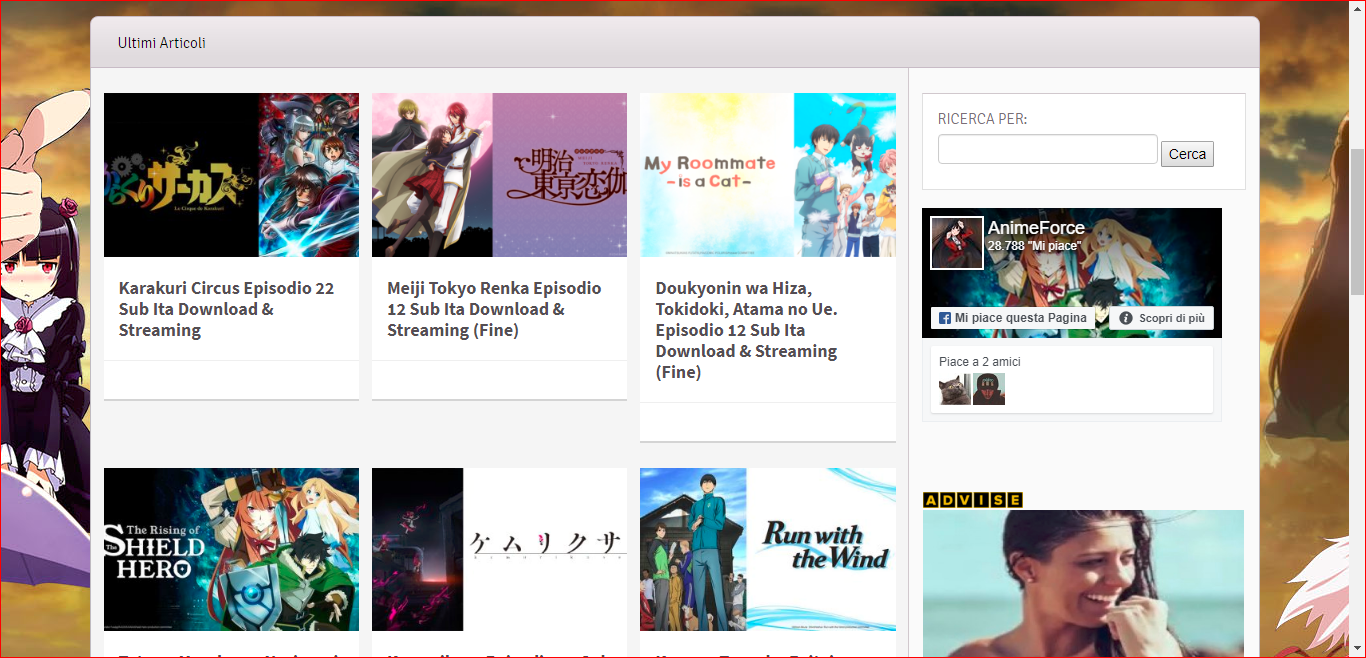
\includegraphics[width=0.5\textwidth]{img/hp02.png}
	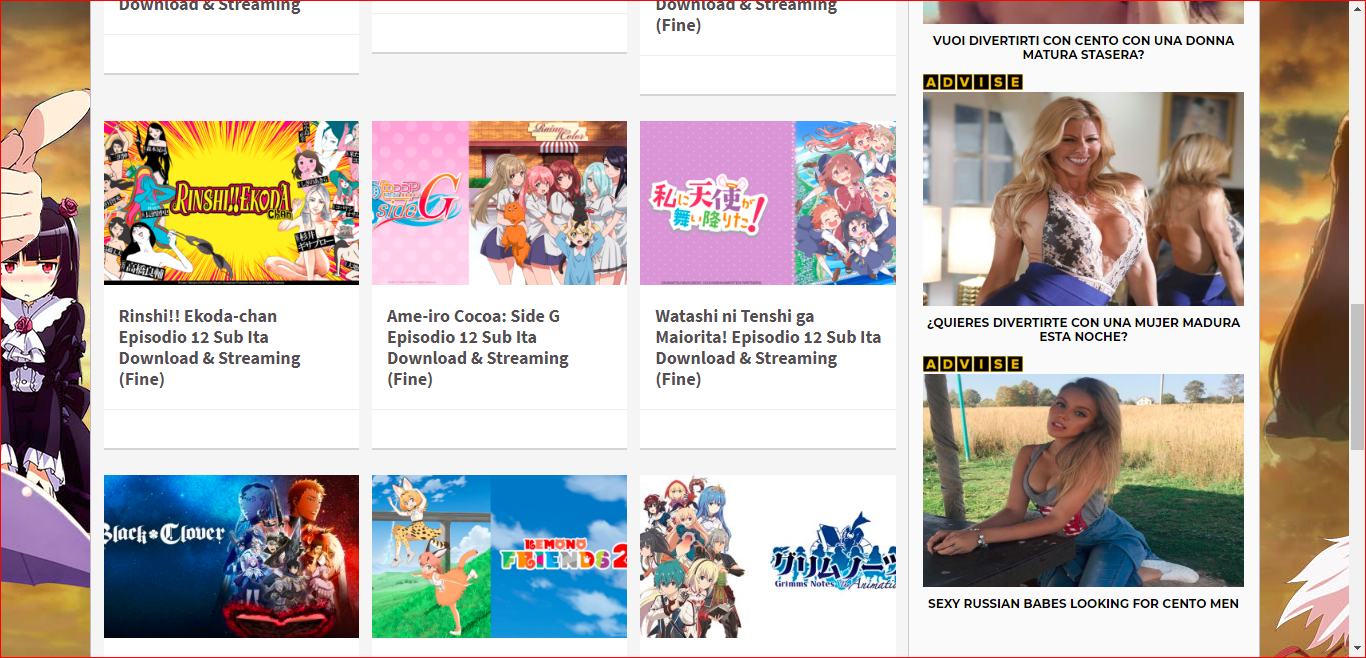
\includegraphics[width=0.5\textwidth]{img/hp03.png}
	\caption{Homepage 1 e 2 scroll} 
	\label{img2} 
\end{figure}

\begin{figure}[H]
	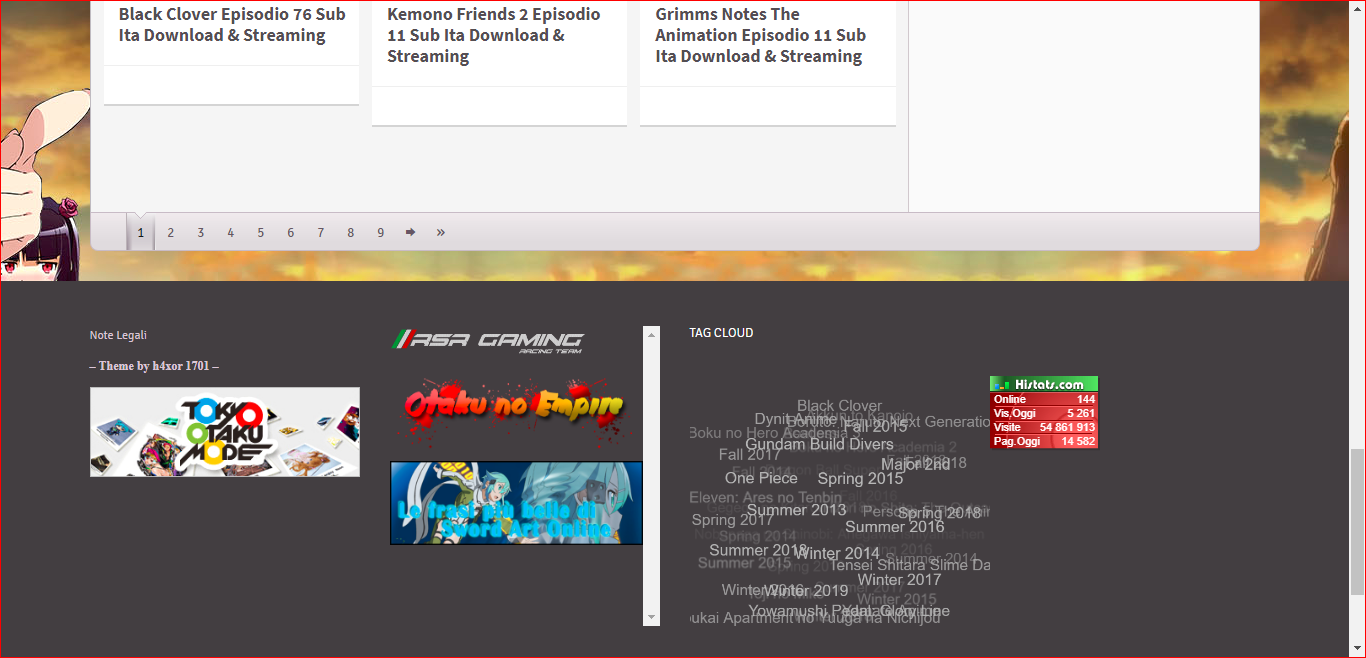
\includegraphics[width=0.5\textwidth]{img/hp04.png}
	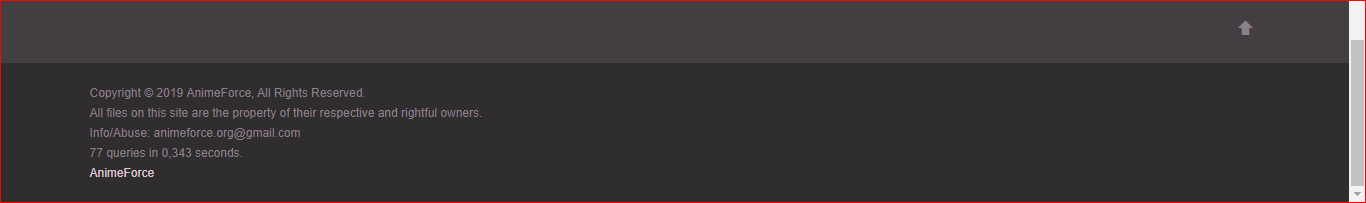
\includegraphics[width=0.5\textwidth]{img/hp05.png}
	\caption{Homepage dopo 3 e 4 scroll} 
	\label{img3} 
\end{figure}

\subsubsection{What - "Che cosa offre il sito?"} \label{HWhat}
Dopo aver effettuato scroll per circa 2,5 pagine il contenuto si compone di immagini preview delle serie animate contenute nel sito in ordine di uscita, dai più recenti a quelli passati. L'offerta abbiamo compreso essere un sito per streaming, ma non vi sono altre informazioni utili, quando in realtà navigando più internamente si comprende la presenza anche di informazioni quali trama, tipologia di anime e numero di serie e se vi sono nuove uscite o i "Coming soon".

\subsubsection{When - "C'è qualche novità?"} \label{HWhen}
La pagina risponde molto bene a questa domanda. Nella homepage sono presenti gli ultimi articoli inseriti e, per ogni nuovo episodio degli anime presenti a catalogo, è possibile scoprirne i nuovi contenuti.
Questo aspetto è molto importante perché permette agli utenti, soprattutto coloro che rientreranno più volte nel sito, di rimanere aggiornati e volendo anche poter ampliare le loro conoscenze su altre serie (oltre a quelle che lo hanno portato a navigare sul sito \nomeSito). La frequenza con cui i nuovi contenuti vengono inseriti nella pagina è sicuramente un punto a favore che gli permette di ottenere fiducia da parte degli utenti abituali e occasionali.

\subsubsection{How - "Come faccio ad arrivare alle sezioni principali?"} \label{HHow}
Per quanto riguarda l' "How" del sito possiamo dire che è facile ed intuitivo; utilizza il menù a tendina per la prima voce a menù (vedi \hyperref[img4]{Figura \ref{img4}}) e le altre due voci, \textit{Contact} e \textit{Chat}, sono semplici link alle pagine di riferimento.
Queste voci sono posizionate in alto alla pagina e l'aspetto negativo è sicuramente che dopo aver effettuato degli scroll verso il basso spariscono. L'utente è costretto ad essere posizionato all'inizio della pagina per poter navigare usando il menù.
Oltre al menù, un altro aspetto legato al come arrivare alle principali sezioni è fornito dalla presenza di una modalità di ricerca in alto a destra e dalla seconda modalità basata sui tag a fondo pagina, che risulta essere però negativa, come andremo a vedere nella sezione Ricerca (\hyperref[Ricerca]{Sezione \ref{Ricerca}}).






